% Options for packages loaded elsewhere
\PassOptionsToPackage{unicode}{hyperref}
\PassOptionsToPackage{hyphens}{url}
\PassOptionsToPackage{dvipsnames,svgnames,x11names}{xcolor}
%
\documentclass[
]{book}
\title{BFW Equilibrium Gender LFP and Wage Code Companion}
\author{Sonia R. Bhalotra, Manuel Fernández, and Fan Wang}
\date{2022-02-15}

\usepackage{amsmath,amssymb}
\usepackage{lmodern}
\usepackage{iftex}
\ifPDFTeX
  \usepackage[T1]{fontenc}
  \usepackage[utf8]{inputenc}
  \usepackage{textcomp} % provide euro and other symbols
\else % if luatex or xetex
  \usepackage{unicode-math}
  \defaultfontfeatures{Scale=MatchLowercase}
  \defaultfontfeatures[\rmfamily]{Ligatures=TeX,Scale=1}
\fi
% Use upquote if available, for straight quotes in verbatim environments
\IfFileExists{upquote.sty}{\usepackage{upquote}}{}
\IfFileExists{microtype.sty}{% use microtype if available
  \usepackage[]{microtype}
  \UseMicrotypeSet[protrusion]{basicmath} % disable protrusion for tt fonts
}{}
\makeatletter
\@ifundefined{KOMAClassName}{% if non-KOMA class
  \IfFileExists{parskip.sty}{%
    \usepackage{parskip}
  }{% else
    \setlength{\parindent}{0pt}
    \setlength{\parskip}{6pt plus 2pt minus 1pt}}
}{% if KOMA class
  \KOMAoptions{parskip=half}}
\makeatother
\usepackage{xcolor}
\IfFileExists{xurl.sty}{\usepackage{xurl}}{} % add URL line breaks if available
\IfFileExists{bookmark.sty}{\usepackage{bookmark}}{\usepackage{hyperref}}
\hypersetup{
  pdftitle={BFW Equilibrium Gender LFP and Wage Code Companion},
  pdfauthor={Sonia R. Bhalotra, Manuel Fernández, and Fan Wang},
  colorlinks=true,
  linkcolor={Maroon},
  filecolor={Maroon},
  citecolor={Blue},
  urlcolor={blue},
  pdfcreator={LaTeX via pandoc}}
\urlstyle{same} % disable monospaced font for URLs
\usepackage{longtable,booktabs,array}
\usepackage{calc} % for calculating minipage widths
% Correct order of tables after \paragraph or \subparagraph
\usepackage{etoolbox}
\makeatletter
\patchcmd\longtable{\par}{\if@noskipsec\mbox{}\fi\par}{}{}
\makeatother
% Allow footnotes in longtable head/foot
\IfFileExists{footnotehyper.sty}{\usepackage{footnotehyper}}{\usepackage{footnote}}
\makesavenoteenv{longtable}
\usepackage{graphicx}
\makeatletter
\def\maxwidth{\ifdim\Gin@nat@width>\linewidth\linewidth\else\Gin@nat@width\fi}
\def\maxheight{\ifdim\Gin@nat@height>\textheight\textheight\else\Gin@nat@height\fi}
\makeatother
% Scale images if necessary, so that they will not overflow the page
% margins by default, and it is still possible to overwrite the defaults
% using explicit options in \includegraphics[width, height, ...]{}
\setkeys{Gin}{width=\maxwidth,height=\maxheight,keepaspectratio}
% Set default figure placement to htbp
\makeatletter
\def\fps@figure{htbp}
\makeatother
\setlength{\emergencystretch}{3em} % prevent overfull lines
\providecommand{\tightlist}{%
  \setlength{\itemsep}{0pt}\setlength{\parskip}{0pt}}
\setcounter{secnumdepth}{5}
\usepackage{bbm}
\usepackage{booktabs}
\usepackage{longtable}
\usepackage{array}
\usepackage{multirow}
\usepackage{wrapfig}
\usepackage{float}
% \floatplacement{figure}{H}
\usepackage[labelformat = empty]{caption}
\usepackage{colortbl}
\usepackage{pdflscape}
\usepackage{tabu}
\usepackage{threeparttable}
\usepackage{threeparttablex}
\usepackage[normalem]{ulem}
\usepackage{makecell}
\usepackage{xcolor}
\usepackage{geometry}
\geometry{
	a4paper,
	left=1.0in,
	right=1.0in,
	top=1.0in,
	bottom=1.0in,
}
\setcounter{secnumdepth}{5}
\setcounter{tocdepth}{5}
\ifLuaTeX
  \usepackage{selnolig}  % disable illegal ligatures
\fi
\usepackage[]{natbib}
\bibliographystyle{apalike}

\begin{document}
\maketitle

{
\hypersetup{linkcolor=}
\setcounter{tocdepth}{1}
\tableofcontents
}
\hypertarget{preface}{%
\chapter*{Preface}\label{preface}}
\addcontentsline{toc}{chapter}{Preface}

This is a work-in-progress Matlab package consisting of functions that solve the equilibrium gender labor force participation and wage model in \href{https://www.iza.org/person/2905/sonia-r-bhalotra}{Bhalotra}, \href{https://sites.google.com/view/manuelfernandezsierra}{Fernández} and \href{https://fanwangecon.github.io/}{Wang} (2022). Tested with \href{https://www.mathworks.com/products/matlab.html}{Matlab} 2021b \citep{matlab}.

All functions are parts of a matlab toolbox that can be installed:

\begin{quote}
Download and install the Matlab toolbox: \href{https://github.com/FanWangEcon/PrjLabEquiBFW/blob/main/PrjLabEquiBFW.mltbx}{PrjLabEquiBFW.mltbx}
\end{quote}

The Code Companion can also be accessed via the bookdown site and PDF linked below:

\begin{quote}
\href{https://fanwangecon.github.io/PrjLabEquiBFW/bookdown/BFW-Equilibrium-Gender-LFP-and-Wage-Code-Companion.pdf}{\textbf{bookdown pdf}}, \href{https://www.mathworks.com/matlabcentral/fileexchange/80164-PrjLabEquiBFW}{\textbf{MathWorks File Exchange}}
\end{quote}

This bookdown file is a collection of mlx based vignettes for functions that are available from \href{https://github.com/FanWangEcon/PrjLabEquiBFW}{PrjLabEquiBFW}. Each Vignette file contains various examples for invoking each function.

The package relies on \href{https://fanwangecon.github.io/MEconTools/}{MEconTools}, which needs to be installed first. The package does not include allocation functions, only simulation code to generate the value of each stimulus check increments for households.

The site is built using \href{https://bookdown.org/}{Bookdown} \citep{R-bookdown}.

Please contact \href{https://fanwangecon.github.io/}{FanWangEcon} for issues or problems.

\hypertarget{introduction}{%
\chapter{Introduction}\label{introduction}}

\hypertarget{bhalotra-fernuxe1ndez-and-wang-2022}{%
\section{Bhalotra, Fernández, and Wang (2022)}\label{bhalotra-fernuxe1ndez-and-wang-2022}}

In Bhalotra, Fernández, and Wang (2022).

\hypertarget{core-functions}{%
\chapter{Core Functions}\label{core-functions}}

\hypertarget{ces-demand-core-functions}{%
\section{CES Demand Core Functions}\label{ces-demand-core-functions}}

This is the example vignette for function:
\href{https://github.com/FanWangEcon/PrjLabEquiBFW/tree/main/PrjLabEquiBFW/func/bfw_mp_func_demand.m}{\textbf{bfw\_mp\_func\_demand}}
from the \href{https://fanwangecon.github.io/PrjLabEquiBFW/}{\textbf{PrjLabEquiBFW
Package}}\textbf{.} This
function generates a container map with key CES demand-side equation for
a particular sub-nest.

\hypertarget{default-test}{%
\subsection{Default Test}\label{default-test}}

Default test

\begin{verbatim}
bl_verbose = true;
mp_func_demand = bfw_mp_func_demand(bl_verbose);

----------------------------------------
xxxxxxxxxxxxxxxxxxxxxxxxxxxxxxxxxxxxxxxx
CONTAINER NAME: mp_func Functions
xxxxxxxxxxxxxxxxxxxxxxxxxxxxxxxxxxxxxxxx
                                i      idx                                                           functionString                                                      
                               ____    ____    __________________________________________________________________________________________________________________________

    fc_OMEGA                   "1"     "1"     "@(p1,p2,rho,beta_1,beta_2)p1.*fc_d1(p1,p2,1,1,rho,beta_1,beta_2)+p2.*fc_d2(p1,p2,1,1,rho,beta_1,beta_2)"                 
    fc_d1                      "2"     "2"     "@(p1,p2,Y,Z,rho,beta_1,beta_2)(Y/Z).*(beta_1+beta_2.*((p1./p2).*(beta_2./beta_1)).^(rho/(1-rho))).^(-1/rho)"             
    fc_d2                      "3"     "3"     "@(p1,p2,Y,Z,rho,beta_1,beta_2)(Y/Z).*(beta_1.*((p2./p1).*(beta_1./beta_2)).^(rho/(1-rho))+beta_2).^(-1/rho)"             
    fc_lagrange_x1             "4"     "4"     "@(p1,rho,beta_1,beta_2,x_1,x_2)p1/(((beta_1*x_1^(rho)+beta_2*x_2^(rho))^((1/rho)-1))*(beta_1*x_1^(rho-1)))"              
    fc_lagrange_x2             "5"     "5"     "@(p2,rho,beta_1,beta_2,x_1,x_2)p2/(((beta_1*x_1^(rho)+beta_2*x_2^(rho))^((1/rho)-1))*(beta_2*x_2^(rho-1)))"              
    fc_output_nest             "6"     "6"     "@(q1,q2,rho,beta_1,beta_2)((beta_1)*q1^(rho)+beta_2*q2^(rho))^(1/rho)"                                                   
    fc_p1_foc                  "7"     "7"     "@(lagrangem,rho,beta_1,beta_2,x_1,x_2)lagrangem*(((beta_1*x_1^(rho)+beta_2*x_2^(rho))^((1/rho)-1))*(beta_1*x_1^(rho-1)))"
    fc_p2_foc                  "8"     "8"     "@(lagrangem,rho,beta_1,beta_2,x_1,x_2)lagrangem*(((beta_1*x_1^(rho)+beta_2*x_2^(rho))^((1/rho)-1))*(beta_2*x_2^(rho-1)))"
    fc_share_given_elas_foc    "9"     "9"     "@(rho,p1,p2,x1,x2)fc_share_given_elas_foc_Q(rho,p1,p2,x1,x2)/(1+fc_share_given_elas_foc_Q(rho,p1,p2,x1,x2))"             
    fc_w1dw2                   "10"    "10"    "@(x_1,x_2,rho,beta_1,beta_2)(x_2/x_1)^(1-rho)*(beta_1/beta_2)"                                                           
    fc_yz_ratio                "11"    "11"    "@(p1,p2,q1,q2,rho,beta_1,beta_2)fc_revenue(p1,p2,q1,q2)/fc_OMEGA(p1,p2,rho,beta_1,beta_2)"                               
\end{verbatim}

\hypertarget{demand}{%
\chapter{Demand}\label{demand}}

\hypertarget{solve-nested-ces-optimal-demand-crs}{%
\section{Solve Nested CES Optimal Demand (CRS)}\label{solve-nested-ces-optimal-demand-crs}}

Testing the
\href{https://github.com/FanWangEcon/PrjLabEquiBFW/blob/main/PrjLabEquiBFW/solvedemand/bfw_crs_nested_ces.m}{\textbf{bfw\_crs\_nested\_ces}}
function from the \href{https://fanwangecon.github.io/PrjLabEquiBFW/}{\textbf{PrjLabEquiBFW
Package}}\textbf{.} This
function solves optimal choices given CES production function under cost
minimization. Works with Constant Elasticity of Substitution problems
with constant returns, up to four nest layers, and two inputs in each
sub-nest. Takes as inputs share and elasticity parameters across layers
of sub-nests, as well as input unit costs at the bottom-most layer.
Works with Constant Elasticity of Substitution problems with constant
returns, up to four nest layers, and two inputs in each sub-nest. Allows
for uneven branches, so that some branches go up to four layers, but
others have less layers, works with BFW (2022) nested labor input
problem.

\hypertarget{key-inputs-and-outputs-for-bfw_mp_func_demand}{%
\subsection{\texorpdfstring{Key Inputs and Outputs for \href{https://github.com/FanWangEcon/PrjLabEquiBFW/tree/main/PrjLabEquiBFW/func/bfw_mp_func_demand.m}{\textbf{bfw\_mp\_func\_demand}}}{Key Inputs and Outputs for bfw\_mp\_func\_demand}}\label{key-inputs-and-outputs-for-bfw_mp_func_demand}}

Here are the key inputs for the CES demand solver function:

\begin{itemize}
\item
  \textbf{FL\_YZ} float output divided by productivity, aggregate single
  term
\item
  \textbf{CL\_MN\_PRHO} cell array of rho (elasticity) parameter between
  negative infinity and 1. For example, suppose there are four nest
  layers, and there are two branches at each layer, then we have 1, 2,
  4, and 8 \(\rho\) parameter values at the 1st, 2nd, 3rd, and 4th nest
  layers: size(CL\_MN\_PRHO\{1\})= \(\left\lbrack 1,1\right\rbrack\),
  size(CL\_MN\_PRHO\{2\}) = \(\left\lbrack 1,2\right\rbrack\),
  size(CL\_MN\_PRHO\{3\}) = \(\left\lbrack 2,2\right\rbrack\),
  size(CL\_MN\_PRHO\{4\}) = \(\left\lbrack 2,2,2\right\rbrack\). Note that
  if the model has 4 nest layers, not all cells need to be specified,
  some branches could be deeper than others.
\item
  \textbf{CL\_MN\_PSHARE} cell array of share (between 0 and 1) for the first
  input of the two inputs for each nest. The structure for this is
  similar to CL\_MN\_PRHO.
\item
  \textbf{CL\_MN\_PRICE} cell array of wages for both wages for the first and
  second nest, the last index in each element of the cell array
  indicates first (1) or second (2) wage. For example, suppose we have
  four layers, with 2 branches at each layer, as in the example for
  CL\_MN\_PRHO, then we have 2, 4, 8, and 16 wage values at the 1st,
  2nd, 3rd, and 4th nest layers: size(CL\_MN\_PRICE\{1\}) =
  \(\left\lbrack 1,2\right\rbrack\), size(CL\_MN\_PRICE\{2\}) =
  \(\left\lbrack 2,2\right\rbrack\), size(CL\_MN\_PRICE\{3\}) =
  \(\left\lbrack 2,2,2\right\rbrack\), size(CL\_MN\_PRICE\{4\}) =
  \(\left\lbrack 2,2,2,2\right\rbrack\) . Note that only the last layer
  of wage needs to be specified, in this case, the 16 wages at the 4th
  layer. Given optimal solutions, we solve for the 2, 4, and 8
  aggregate wages at the higher nest layers. If some branches are
  deeper than other branches, then can specific NA for non-reached
  layers along some branches.
\item
  \textbf{BL\_BFW\_MODEL} boolean true by default if true then will output
  outcomes specific to the BFW 2022 problem.
\end{itemize}

Here are the key outputs for the CES demand solver function:

\begin{itemize}
\item
  \textbf{CL\_MN\_YZ\_CHOICES} has the same dimension as CL\_MN\_PRICE, suppose
  there are four layers, the CL\_MN\_PRICE\{4\} results at the lowest
  layer includes quantity choices that might be observed in the data.
  CL\_MN\_PRICE cell values at non-bottom layers include aggregate
  quantity outcomes.
\item
  \textbf{CL\_MN\_PRICE} includes at the lowest layer observed wages,
  however, also includes higher layer aggregate solved waves.
  CL\_MN\_PRHO and CL\_MN\_PSHARE are identical to inputs.
\end{itemize}

\hypertarget{single-nest-layer-two-inputs-ces-problem-demand}{%
\subsection{Single Nest Layer Two Inputs CES Problem (Demand)}\label{single-nest-layer-two-inputs-ces-problem-demand}}

In this first example, we solve a constant returns to scale problem with
a single nest, meaning just two inputs and a single output.

\begin{verbatim}
clc;
close all;
clear all;

% Output requirement
fl_yz = 1;
% rho = 0.5, 1/(1-0.5)=2, elasticity of substitution of 2
cl_mn_prho = {[0.1]};
% equal share, similar "productivity"
cl_mn_pshare = {[0.5]};
% wages for the two inputs, identical wage
cl_mn_price = {[1.5, 0.75]};
% print option
bl_verbose = true;
mp_func = bfw_mp_func_demand();
bl_bfw_model = false;
[cl_mn_yz_choices, cl_mn_price] = ...
    bfw_crs_nested_ces(fl_yz, cl_mn_prho, cl_mn_pshare, cl_mn_price, ...
    mp_func, bl_verbose, bl_bfw_model);

----------------------------------------
xxxxxxxxxxxxxxxxxxxxxxxxxxxxxxxxxxxxxxxx
CONTAINER NAME: mp_container_map ND Array (Matrix etc)
xxxxxxxxxxxxxxxxxxxxxxxxxxxxxxxxxxxxxxxx
                i    idx    ndim    numel    rowN    colN     sum       mean       std      coefvari      min       max  
                _    ___    ____    _____    ____    ____    ______    ______    _______    ________    _______    ______

    price_c1    1     2      2        2       1       2        2.25     1.125    0.53033     0.4714        0.75       1.5
    yz_c1       2     4      2        2       1       2      2.1343    1.0671    0.55403    0.51918     0.67537    1.4589

xxx TABLE:price_c1 xxxxxxxxxxxxxxxxxx
          c1      c2 
          ___    ____

    r1    1.5    0.75

xxx TABLE:yz_c1 xxxxxxxxxxxxxxxxxx
            c1         c2  
          _______    ______

    r1    0.67537    1.4589

----------------------------------------
xxxxxxxxxxxxxxxxxxxxxxxxxxxxxxxxxxxxxxxx
CONTAINER NAME: mp_container_map Scalars
xxxxxxxxxxxxxxxxxxxxxxxxxxxxxxxxxxxxxxxx
                 i    idx    value
                 _    ___    _____

    prho_c1      1     1      0.1 
    pshare_c1    2     3      0.5 
\end{verbatim}

\hypertarget{single-nest-layer-two-inputs-ces-problem-vary-share-and-elasticity-demand}{%
\subsection{Single Nest Layer Two Inputs CES Problem, Vary Share and Elasticity (Demand)}\label{single-nest-layer-two-inputs-ces-problem-vary-share-and-elasticity-demand}}

In this second example, we test over different rho values, explore
optimal relative choices, as share and elasticity change. In this
exercise, we also check, at every combination of rho and share
parameter, whether the FOC condition is satisfied by the optimal
choices. Also check if at the optimal choices, the minimization output
requirement is met.

\begin{verbatim}
% Approximately close function
rel_tol=1e-09;
abs_tol=0.0;
if_is_close = @(a,b) (abs(a-b) <= max(rel_tol * max(abs(a), abs(b)), abs_tol));

% Define share and rho arrays
fl_yz = 1;
ar_pshare = linspace(0.1, 0.9, 9);
ar_prho = 1 - 10.^(linspace(-2, 2, 30));
% Loop over share and rho values
mt_rela_opti = NaN([length(ar_pshare), length(ar_prho)]);
mt_x1_opti = NaN([length(ar_pshare), length(ar_prho)]);
for it_pshare_ctr = 1:length(ar_pshare)
    for it_prho_ctr = 1:length(ar_prho)

        % A. Parameters
        % rho
        fl_prho = ar_prho(it_prho_ctr);
        cl_mn_prho = {[fl_prho]};
        % share
        fl_pshare = ar_pshare(it_pshare_ctr);
        cl_mn_pshare = {[fl_pshare]};
        % wages for the two inputs, identical wage
        cl_mn_price = {[1, 1]};
        % print option
        bl_verbose = false;

        % B. Call function
        [cl_mn_yz_choices, cl_mn_price, cl_mn_prho, cl_mn_pshare] = ...
            bfw_crs_nested_ces(fl_yz, cl_mn_prho, cl_mn_pshare, cl_mn_price, ...
            mp_func, bl_verbose, bl_bfw_model);
        % Store results for optimal choice
        fl_opti_x1 = cl_mn_yz_choices{1}(1);
        fl_opti_x2 = cl_mn_yz_choices{1}(2);
        mt_x1_opti(it_pshare_ctr, it_prho_ctr) = fl_opti_x1;

        % C. Check if relative optimality FOC condition is met
        fl_rela_opti = fl_opti_x1/fl_opti_x2;
        % From FOC give wages = 1 both
        % Using What is above Equation A.20 in draft.
        fl_rela_opti_foc = (((fl_pshare/(1-fl_pshare)))*(1))^(1/(1-ar_prho(it_prho_ctr)));
        if (~if_is_close(fl_rela_opti_foc, fl_rela_opti))
            error('There is an error, optimal relative not equal to expected foc ratio')
        end

        % D. Check if output quantity requirement is met
        fl_output = ((fl_pshare)*fl_opti_x1^(fl_prho) + (1-fl_pshare)*fl_opti_x2^(fl_prho))^(1/fl_prho);
        if (~if_is_close(fl_output, fl_yz))
            error('There is an error, output is not equal to required expenditure minimizing output')
        end

    end
end
\end{verbatim}

Key results: (1) As share parameter of input 1 goes to zero, optimal
choice goes to zero when inputs are elastic; (2) When inputs are
inelasticty, even very low share input 1 asymptote to equal input 2; (3)
When input 1 is more productive (higher share), actually hire less as
productivity (share) increases, becasue less of it is needed to achieve
production for high rho, elastictic production function; (4) For
inelastic production, monotonic relationship between input and shares.

\begin{verbatim}
% Visualize
% Generate some Data
rng(456);
ar_row_grid = ar_pshare;
ar_col_grid = log(1-ar_prho)/log(10);
rng(123);
mt_value = mt_x1_opti;
% container map settings
mp_support_graph = containers.Map('KeyType', 'char', 'ValueType', 'any');
mp_support_graph('cl_st_graph_title') = {'Optimal input 1 choice, rho=x, share=color'};
mp_support_graph('cl_st_ytitle') = {'Optimal choice of input 1'};
mp_support_graph('cl_st_xtitle') = {'Rho in (1-log10(rho)) scale', ...
    'left = perfect substitution (rho = 1)', ...
    'right = perfect complements (negative infinity rho)'};
mp_support_graph('st_legend_loc') = 'southwest';
mp_support_graph('bl_graph_logy') = false; % do not log
mp_support_graph('st_rowvar_name') = 'share=';
mp_support_graph('it_legend_select') = 5; % how many shock legends to show
mp_support_graph('st_rounding') = '6.3f'; % format shock legend
mp_support_graph('cl_colors') = 'jet'; % any predefined matlab colormap
% Call function
ff_graph_grid(mt_value, ar_row_grid, ar_col_grid, mp_support_graph);
\end{verbatim}

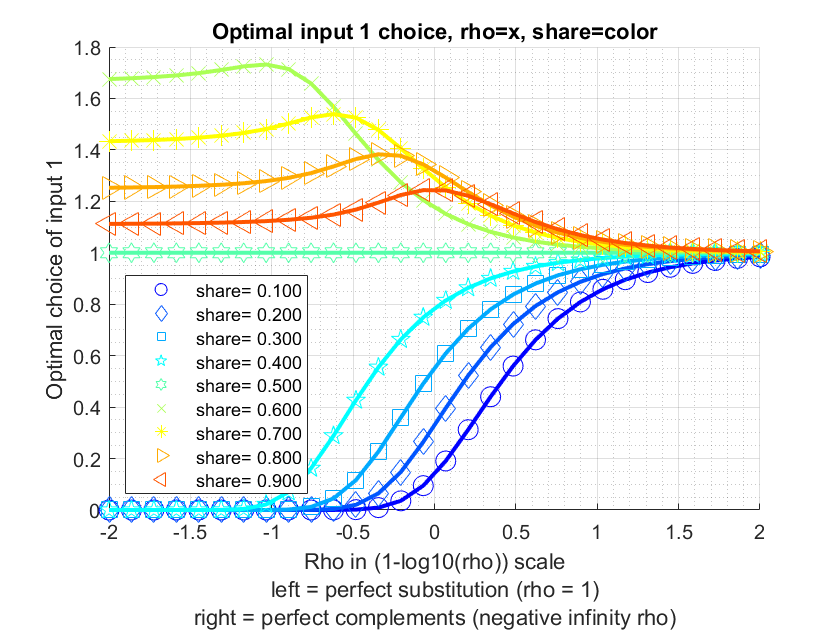
\includegraphics[width=5.20833in,height=\textheight]{img/bfwx_crs_nested_ces_images/figure_0.png}

\hypertarget{doubly-nest-layer-two-inputs-each-sub-nest-ces-problem-demand}{%
\subsection{Doubly Nest Layer Two Inputs Each Sub-nest CES Problem (Demand)}\label{doubly-nest-layer-two-inputs-each-sub-nest-ces-problem-demand}}

In this third example, solve for optimal choices for a doubly nested
problem. Below, we first solve for the optimal choices, then we do a
number of checks, to make sure that the solutions are correct, as
expected.

\begin{verbatim}
% output requirement
fl_yz = 2.1;
% upper nest 0.1, lower nests 0.35 and -1 separately for rho values
cl_mn_prho = {[0.1], [0.35, -1]};
% unequal shares of share values
cl_mn_pshare = {[0.4], [0.3, 0.88]};
% differential wages
% in lower-left nest, not productive and very expensive, not very elastic
% last index for left or right,
cl_mn_price = {[nan, nan], [10, 1;3, 4]};
% print option
bl_verbose = true;
[cl_mn_yz_choices, cl_mn_price, cl_mn_prho, cl_mn_pshare] = ...
    bfw_crs_nested_ces(fl_yz, cl_mn_prho, cl_mn_pshare, cl_mn_price, ...
    mp_func, bl_verbose, bl_bfw_model);

----------------------------------------
xxxxxxxxxxxxxxxxxxxxxxxxxxxxxxxxxxxxxxxx
CONTAINER NAME: mp_container_map ND Array (Matrix etc)
xxxxxxxxxxxxxxxxxxxxxxxxxxxxxxxxxxxxxxxx
                 i    idx    ndim    numel    rowN    colN     sum       mean       std      coefvari      min        max  
                 _    ___    ____    _____    ____    ____    ______    ______    _______    ________    ________    ______

    prho_c2      1     2      2        2       1       2       -0.65    -0.325    0.95459    -2.9372           -1      0.35
    price_c1     2     3      2        2       1       2      7.7788    3.8894     2.0959    0.53886       2.4074    5.3714
    price_c2     3     4      2        4       2       2          18       4.5      3.873    0.86066            1        10
    pshare_c2    4     6      2        2       1       2        1.18      0.59    0.41012    0.69512          0.3      0.88
    yz_c1        5     7      2        2       1       2      4.4862    2.2431    0.68863      0.307       1.7561      2.73
    yz_c2        6     8      2        4       2       2      9.0506    2.2626     2.7086     1.1971     0.047893    6.0934

xxx TABLE:prho_c2 xxxxxxxxxxxxxxxxxx
           c1     c2
          ____    __

    r1    0.35    -1

xxx TABLE:price_c1 xxxxxxxxxxxxxxxxxx
            c1        c2  
          ______    ______

    r1    2.4074    5.3714

xxx TABLE:price_c2 xxxxxxxxxxxxxxxxxx
          c1    c2
          __    __

    r1    10    1 
    r2     3    4 

xxx TABLE:pshare_c2 xxxxxxxxxxxxxxxxxx
          c1      c2 
          ___    ____

    r1    0.3    0.88

xxx TABLE:yz_c1 xxxxxxxxxxxxxxxxxx
           c1       c2  
          ____    ______

    r1    2.73    1.7561

xxx TABLE:yz_c2 xxxxxxxxxxxxxxxxxx
             c1         c2   
          ________    _______

    r1    0.047893     6.0934
    r2      2.2044    0.70496

----------------------------------------
xxxxxxxxxxxxxxxxxxxxxxxxxxxxxxxxxxxxxxxx
CONTAINER NAME: mp_container_map Scalars
xxxxxxxxxxxxxxxxxxxxxxxxxxxxxxxxxxxxxxxx
                 i    idx    value
                 _    ___    _____

    prho_c1      1     1      0.1 
    pshare_c1    2     5      0.4 

% there are four optimal choices, they are
fl_opti_x11 = cl_mn_yz_choices{2}(1,1);
fl_opti_x12 = cl_mn_yz_choices{2}(1,2);
fl_opti_x21 = cl_mn_yz_choices{2}(2,1);
fl_opti_x22 = cl_mn_yz_choices{2}(2,2);
% display
st_print = strjoin(...
    ["completed double nest test:", ...
    ['nest 1 input 1, fl_opti_x11=' num2str(fl_opti_x11)], ...
    ['nest 1 input 2, fl_opti_x12=' num2str(fl_opti_x12)], ...
    ['nest 2 input 1, fl_opti_x21=' num2str(fl_opti_x21)], ...
    ['nest 2 input 2, fl_opti_x22=' num2str(fl_opti_x22)], ...
    ], ";");
st_out = st_print;
ar_ch_out = char(strsplit(st_print,";")');
disp(ar_ch_out);

completed double nest test:         
nest 1 input 1, fl_opti_x11=0.047893
nest 1 input 2, fl_opti_x12=6.0934  
nest 2 input 1, fl_opti_x21=2.2044  
nest 2 input 2, fl_opti_x22=0.70496 
\end{verbatim}

\hypertarget{doubly-nest-layer-two-inputs-each-sub-nest-ces-problemsolution-check-demand}{%
\subsection{Doubly Nest Layer Two Inputs Each Sub-nest CES Problem--Solution Check (Demand)}\label{doubly-nest-layer-two-inputs-each-sub-nest-ces-problemsolution-check-demand}}

Checking output equality, if there are problems, would output an error.

\begin{verbatim}
% A. Check output Equality
fl_pshare_0 = cl_mn_pshare{1}(1);
fl_pshare_1 = cl_mn_pshare{2}(1);
fl_pshare_2 = cl_mn_pshare{2}(2);
fl_prho_0 = cl_mn_prho{1}(1);
fl_prho_1 = cl_mn_prho{2}(1);
fl_prho_2 = cl_mn_prho{2}(2);
fl_output_1 = ((fl_pshare_1)*fl_opti_x11^(fl_prho_1) + (1-fl_pshare_1)*fl_opti_x12^(fl_prho_1))^(1/fl_prho_1);
fl_output_2 = ((fl_pshare_2)*fl_opti_x21^(fl_prho_2) + (1-fl_pshare_2)*fl_opti_x22^(fl_prho_2))^(1/fl_prho_2);
fl_output_0 = ((fl_pshare_0)*fl_output_1^(fl_prho_0) + (1-fl_pshare_0)*fl_output_2^(fl_prho_0))^(1/fl_prho_0);
if (~if_is_close(fl_output_0, fl_yz))
    error('There is an error, output is not equal to required expenditure minimizing output')
end
\end{verbatim}

Checking FOC within-nest optimality, if there are problems, would output
an error.

\begin{verbatim}
% B. Check FOC Optimality inner nest
fl_wage_x11 = cl_mn_price{2}(1,1);
fl_wage_x12 = cl_mn_price{2}(1,2);
fl_wage_x21 = cl_mn_price{2}(2,1);
fl_wage_x22 = cl_mn_price{2}(2,2);

% B1. Checking via Method 1
fl_rela_opti_foc_1 = (((fl_pshare_1/(1-fl_pshare_1)))*(fl_wage_x12/fl_wage_x11))^(1/(1-fl_prho_1));
fl_rela_opti_foc_2 = (((fl_pshare_2/(1-fl_pshare_2)))*(fl_wage_x22/fl_wage_x21))^(1/(1-fl_prho_2));
if (~if_is_close(fl_rela_opti_foc_1, fl_opti_x11/fl_opti_x12))
    error('B1. There is an error, optimal relative not equal to expected foc ratio, nest 1')
end
if (~if_is_close(fl_rela_opti_foc_2, fl_opti_x21/fl_opti_x22))
    error('B1. There is an error, optimal relative not equal to expected foc ratio, nest 2')
end

% B2. Equation left to right, right to left, checking via method 2
% Check FOC Optimality cross nests (actually within) T1
fl_dy_dx11 = fl_pshare_1*(fl_opti_x11^(fl_prho_1-1));
fl_dy_dx12 = (1-fl_pshare_1)*(fl_opti_x12^(fl_prho_1-1));
fl_rwage_x11dx12 = fl_dy_dx11/fl_dy_dx12;
if (~if_is_close(fl_rwage_x11dx12, fl_wage_x11/fl_wage_x12))
    error('B2. There is an error, relative price x11 and x12 does not satisfy within optimality across nests')
end
\end{verbatim}

Generate aggregate prices, if there are problems, would output an error.

\begin{verbatim}
% C. Aggregate prices and optimality within higher tier
% Is optimality satisfied given aggregate prices?
fl_rela_wage_share_11 = ...
    ((fl_wage_x11/fl_wage_x12)*((1-fl_pshare_1)/(fl_pshare_1)))^(fl_prho_1/(1-fl_prho_1));
fl_rela_wage_share_12 = ...
    ((fl_wage_x12/fl_wage_x11)*((fl_pshare_1)/(1-fl_pshare_1)))^(fl_prho_1/(1-fl_prho_1));
fl_agg_prc_1 = ...
    fl_wage_x11*(fl_pshare_1 + (1-fl_pshare_1)*(fl_rela_wage_share_11))^(-1/fl_prho_1) + ...
    fl_wage_x12*(fl_pshare_1*(fl_rela_wage_share_12) + (1-fl_pshare_1))^(-1/fl_prho_1);

fl_rela_wage_share_21 = ...
    ((fl_wage_x21/fl_wage_x22)*((1-fl_pshare_2)/(fl_pshare_2)))^(fl_prho_2/(1-fl_prho_2));
fl_rela_wage_share_22 = ...
    ((fl_wage_x22/fl_wage_x21)*((fl_pshare_2)/(1-fl_pshare_2)))^(fl_prho_2/(1-fl_prho_2));
fl_agg_prc_2 = ...
    fl_wage_x21*(fl_pshare_2 + (1-fl_pshare_2)*(fl_rela_wage_share_21))^(-1/fl_prho_2) + ...
    fl_wage_x22*(fl_pshare_2*(fl_rela_wage_share_22) + (1-fl_pshare_2))^(-1/fl_prho_2);

% What is returned by the omega function that is suppose to have aggregate prices?
mp_func = bfw_mp_func_demand();
params_group = values(mp_func, {'fc_OMEGA', 'fc_d1', 'fc_d2'});
[fc_OMEGA, fc_d1, fc_d2] = params_group{:};

% Aggregate price
fl_aggregate_price_1 = fc_OMEGA(...
    fl_wage_x11, fl_wage_x12, ...
    fl_prho_1, ...
    fl_pshare_1, 1 - fl_pshare_1);

fl_aggregate_price_2 = fc_OMEGA(...
    fl_wage_x21, fl_wage_x22, ...
    fl_prho_2, ...
    fl_pshare_2, 1 - fl_pshare_2);    
\end{verbatim}

Check relative price within nest and across nests, if there are
problems, would output an error.

\begin{verbatim}
% D. Check FOC Optimality cross nests

% D1a. Two within-nest relative wages and four cross-nest relative wages
% within
fl_rwage_x11dx12 = fl_wage_x11/fl_wage_x12;
fl_rwage_x21dx22 = fl_wage_x21/fl_wage_x22;
% across
fl_rwage_x11dx21 = fl_wage_x11/fl_wage_x21;
fl_rwage_x11dx22 = fl_wage_x11/fl_wage_x22;
fl_rwage_x12dx21 = fl_wage_x12/fl_wage_x21;
fl_rwage_x12dx22 = fl_wage_x12/fl_wage_x22;

% D1b. Generate relative wages within nest and across nests own equations
fl_dy_dx1_shared = (fl_pshare_0*(fl_output_1)^(fl_prho_0-1))*((fl_output_1)^(1-fl_prho_1));
fl_dy_dx11 = fl_dy_dx1_shared*(fl_pshare_1*fl_opti_x11^(fl_prho_1-1));
fl_dy_dx12 = fl_dy_dx1_shared*((1-fl_pshare_1)*fl_opti_x12^(fl_prho_1-1));

fl_dy_dx2_shared = ((1-fl_pshare_0)*(fl_output_2)^(fl_prho_0-1))*((fl_output_2)^(1-fl_prho_2));
fl_dy_dx21 = fl_dy_dx2_shared*(fl_pshare_2*fl_opti_x21^(fl_prho_2-1));
fl_dy_dx22 = fl_dy_dx2_shared*((1-fl_pshare_2)*fl_opti_x22^(fl_prho_2-1));

% within
fl_rwage_x11dx12_foc = fl_dy_dx11/fl_dy_dx12;
fl_rwage_x21dx22_foc = fl_dy_dx21/fl_dy_dx22;
% across
fl_rwage_x11dx21_foc = fl_dy_dx11/fl_dy_dx21;
fl_rwage_x11dx22_foc = fl_dy_dx11/fl_dy_dx22;
fl_rwage_x12dx21_foc = fl_dy_dx12/fl_dy_dx21;
fl_rwage_x12dx22_foc = fl_dy_dx12/fl_dy_dx22;

if (~if_is_close(fl_rwage_x11dx21_foc, fl_wage_x11/fl_wage_x21))
    error('There is an error, relative price x11 and x21 does not satisfy cross optimality across nests')
end
if (~if_is_close(fl_rwage_x12dx22_foc, fl_wage_x12/fl_wage_x22))
    error('There is an error, relative price x12 and x22 does not satisfy cross optimality across nests')
end

% D2. Check FOC Optimality cross nests, simplified equation
fl_rela_wage_x11_x21 = log((fl_pshare_0/(1-fl_pshare_0))* ...
    ((fl_pshare_1*fl_opti_x11^(fl_prho_1-1)*fl_output_2^(fl_prho_2))/(fl_pshare_2*fl_opti_x21^(fl_prho_2-1)*fl_output_1^(fl_prho_1)))) + ...
    fl_prho_0*log(fl_output_1/fl_output_2);
if (~if_is_close(fl_rela_wage_x11_x21, log(fl_wage_x11/fl_wage_x21)))
    error('There is an error, relative price x11 and x21 does not satisfy cross optimality across nests')
end
\end{verbatim}

\hypertarget{bfw-2022-nested-three-branch-four-layer-problem-demand}{%
\subsection{BFW (2022) Nested Three Branch (Four Layer) Problem (Demand)}\label{bfw-2022-nested-three-branch-four-layer-problem-demand}}

The model BFW 2022 has three branches and four layers. one of the
branches go down only three layers, the other two branches go down four
layers.

First, we prepare the various inputs:

\begin{verbatim}
% Controls
bl_verbose = true;
bl_bfw_model = true;

% Given rho and beta, solve for equilibrium quantities
bl_log_wage = false;
mp_func = bfw_mp_func_demand(bl_log_wage);

% Following instructions in: PrjFLFPMexicoBFW\solvedemand\README.md

% Nests/layers
it_nests = 4;

% Input cell of mn matrixes
it_prho_cl = 1;
it_pshare_cl = 2;
it_price_cl = 3;
for it_cl_ctr = [1,2,3]

    cl_mn_cur = cell(it_nests,1);

    % Fill each cell element with NaN mn array
    for it_cl_mn = 1:it_nests

        bl_price = (it_cl_ctr == it_price_cl);

        if (~bl_price && it_cl_mn == 1)
            mn_nan = NaN;
        elseif (~bl_price && it_cl_mn == 2) || (bl_price && it_cl_mn == 1)
            mn_nan = [NaN, NaN];
        elseif (~bl_price && it_cl_mn == 3) || (bl_price && it_cl_mn == 2)
            mn_nan = NaN(2,2);
        elseif (~bl_price && it_cl_mn == 4) || (bl_price && it_cl_mn == 3)
            mn_nan = NaN(2,2,2);
        elseif (~bl_price && it_cl_mn == 5) || (bl_price && it_cl_mn == 4)
            mn_nan = NaN(2,2,2,2);
        elseif (~bl_price && it_cl_mn == 6) || (bl_price && it_cl_mn == 5)
            mn_nan = NaN(2,2,2,2,2);
        end
        cl_mn_cur{it_cl_mn} = mn_nan;
    end

    % Name cell arrays
    if (it_cl_ctr == it_prho_cl)
        cl_mn_prho = cl_mn_cur;
    elseif (it_cl_ctr == it_pshare_cl)
        cl_mn_pshare = cl_mn_cur;
    elseif (it_cl_ctr == it_price_cl)
        cl_mn_price = cl_mn_cur;
    end
end

% Initialize share matrix
rng(123);
for it_cl_mn = 1:it_nests
    mn_pshare = cl_mn_pshare{it_cl_mn};
    if it_cl_mn == 4
        mn_pshare(2,:,:) = rand(2,2);
    else
        mn_pshare = rand(size(mn_pshare));
    end
    cl_mn_pshare{it_cl_mn} = mn_pshare;
end

% Initialize rho matrix
rng(456);
for it_cl_mn = 1:it_nests
    mn_prho = cl_mn_prho{it_cl_mn};
    if it_cl_mn == 4
        mn_prho(2,:,:) = rand(2,2);
    else
        mn_prho = rand(size(mn_prho));
    end
    % Scalling rho between 0.7500 and -3.0000
    % 1 - 2.^(linspace(-2,2,5))
    mn_prho = 1 - 2.^(mn_prho*(4) - 2);
    cl_mn_prho{it_cl_mn} = mn_prho;
end

% Initialize wage matrix
rng(789);
for it_cl_mn = 1:it_nests
    mn_price = cl_mn_price{it_cl_mn};
    if it_cl_mn == 3
        mn_price(1,:,:) = rand(2,2);
    elseif it_cl_mn == 4
        mn_price(2,:,:,:) = rand(2,2,2);
    end
    % Scalling rho between 3 amd 5
    mn_price = mn_price*(2) + 3;
    cl_mn_price{it_cl_mn} = mn_price;
end

% Initialize yz matrix
rng(101112);
fl_yz = rand();
\end{verbatim}

Second, display created inputs:

\begin{verbatim}
disp(['fl_yz=' num2str(fl_yz)]);

fl_yz=0.89726

celldisp(cl_mn_prho);

cl_mn_prho
 
cl_mn_prho{1} =
 
    0.5017



cl_mn_prho{2} =
 
    0.6071   -1.1955



cl_mn_prho{3} =
 
   -1.3523   -0.3346
   -0.4167   -1.9136



cl_mn_prho{4} =
 

(:,:,1) =

       NaN       NaN
   -1.0512    0.5869


(:,:,2) =

       NaN       NaN
    0.6209    0.1633



celldisp(cl_mn_pshare);

cl_mn_pshare
 
cl_mn_pshare{1} =
 
    0.6965



cl_mn_pshare{2} =
 
    0.2861    0.2269



cl_mn_pshare{3} =
 
    0.5513    0.4231
    0.7195    0.9808



cl_mn_pshare{4} =
 

(:,:,1) =

       NaN       NaN
    0.6848    0.4809


(:,:,2) =

       NaN       NaN
    0.3921    0.3432



celldisp(cl_mn_price);

cl_mn_price
 
cl_mn_price{1} =
 
   NaN   NaN



cl_mn_price{2} =
 
   NaN   NaN
   NaN   NaN



cl_mn_price{3} =
 

(:,:,1) =

    3.6467    3.4605
       NaN       NaN


(:,:,2) =

    4.5876    4.2488
       NaN       NaN



cl_mn_price{4} =
 

(:,:,1,1) =

       NaN       NaN
    4.9508    4.5178


(:,:,2,1) =

       NaN       NaN
    3.0212    3.0495


(:,:,1,2) =

       NaN       NaN
    3.2221    4.0763


(:,:,2,2) =

       NaN       NaN
    3.0909    4.1031
\end{verbatim}

Third, call function and solve for optimal demand:

\begin{verbatim}
% Call function
[cl_mn_yz_choices, cl_mn_price, cl_mn_prho, cl_mn_pshare] = ...
    bfw_crs_nested_ces(fl_yz, cl_mn_prho, cl_mn_pshare, cl_mn_price, ...
    mp_func, bl_verbose, bl_bfw_model);

----------------------------------------
xxxxxxxxxxxxxxxxxxxxxxxxxxxxxxxxxxxxxxxx
CONTAINER NAME: mp_container_map ND Array (Matrix etc)
xxxxxxxxxxxxxxxxxxxxxxxxxxxxxxxxxxxxxxxx
                            i     idx    ndim    numel    rowN    colN      sum         mean        std       coefvari      min         max   
                            __    ___    ____    _____    ____    ____    ________    ________    ________    ________    ________    ________

    mt_fl_labor_demanded     1     1      2       12       4       3        5.4455     0.45379     0.85359       1.881    0.020122      2.3642
    prho_c2                  2     3      2        2       1       2      -0.58844    -0.29422      1.2746     -4.3323     -1.1955     0.60709
    prho_c3                  3     4      2        4       2       2       -4.0173     -1.0043     0.76195    -0.75868     -1.9136    -0.33464
    prho_c4                  4     5      3        8       2       4           NaN         NaN         NaN         NaN     -1.0512     0.62089
    price_c1                 5     6      2        2       1       2        35.345      17.673      7.0394     0.39832      12.695       22.65
    price_c2                 6     7      2        4       2       2        40.906      10.226      2.7834     0.27217      7.7015      13.522
    price_c3                 7     8      3        8       2       4        45.403      5.6754      2.0037     0.35305      3.4605      8.5114
    price_c4                 8     9      4       16       2       8           NaN         NaN         NaN         NaN      3.0212      4.9508
    pshare_c2                9    11      2        2       1       2       0.51299      0.2565    0.041923     0.16344     0.22685     0.28614
    pshare_c3               10    12      2        4       2       2        2.6747     0.66866     0.24087     0.36023     0.42311     0.98076
    pshare_c4               11    13      3        8       2       4           NaN         NaN         NaN         NaN     0.34318     0.68483
    yz_c1                   12    14      2        2       1       2        1.6003     0.80016      1.0053      1.2564    0.089284       1.511
    yz_c2                   13    15      2        4       2       2         2.645     0.66124      1.0849      1.6407    0.057461      2.2864
    yz_c3                   14    16      3        8       2       4        5.1962     0.64953      1.0063      1.5492     0.03298      2.3642
    yz_c4                   15    17      4       16       2       8           NaN         NaN         NaN         NaN    0.020122     0.14469

xxx TABLE:mt_fl_labor_demanded xxxxxxxxxxxxxxxxxx
             c1          c2         c3   
          ________    ________    _______

    r1    0.020122    0.024929     2.1857
    r2    0.060227    0.037985     2.3642
    r3    0.069088    0.093774    0.21107
    r4    0.058349     0.14469    0.17539

xxx TABLE:prho_c2 xxxxxxxxxxxxxxxxxx
            c1         c2   
          _______    _______

    r1    0.60709    -1.1955

xxx TABLE:prho_c3 xxxxxxxxxxxxxxxxxx
             c1          c2   
          ________    ________

    r1     -1.3523    -0.33464
    r2    -0.41668     -1.9136

xxx TABLE:prho_c4 xxxxxxxxxxxxxxxxxx
            c1         c2         c3         c4   
          _______    _______    _______    _______

    r1        NaN        NaN        NaN        NaN
    r2    -1.0512    0.58694    0.62089    0.16334

xxx TABLE:price_c1 xxxxxxxxxxxxxxxxxx
            c1       c2  
          ______    _____

    r1    12.695    22.65

xxx TABLE:price_c2 xxxxxxxxxxxxxxxxxx
            c1        c2  
          ______    ______

    r1    8.1518    7.7015
    r2    13.522     11.53

xxx TABLE:price_c3 xxxxxxxxxxxxxxxxxx
            c1        c2        c3        c4  
          ______    ______    ______    ______

    r1    3.6467    3.4605    4.5876    4.2488
    r2    8.1184    8.5114    5.7986    7.0309

xxx TABLE:price_c4 xxxxxxxxxxxxxxxxxx
            c1        c2        c3        c4        c5        c6        c7        c8  
          ______    ______    ______    ______    ______    ______    ______    ______

    r1       NaN       NaN       NaN       NaN       NaN       NaN       NaN       NaN
    r2    4.9508    4.5178    3.0212    3.0495    3.2221    4.0763    3.0909    4.1031

xxx TABLE:pshare_c2 xxxxxxxxxxxxxxxxxx
            c1         c2   
          _______    _______

    r1    0.28614    0.22685

xxx TABLE:pshare_c3 xxxxxxxxxxxxxxxxxx
            c1         c2   
          _______    _______

    r1    0.55131    0.42311
    r2    0.71947    0.98076

xxx TABLE:pshare_c4 xxxxxxxxxxxxxxxxxx
            c1         c2         c3         c4   
          _______    _______    _______    _______

    r1        NaN        NaN        NaN        NaN
    r2    0.68483    0.48093    0.39212    0.34318

xxx TABLE:yz_c1 xxxxxxxxxxxxxxxxxx
           c1         c2   
          _____    ________

    r1    1.511    0.089284

xxx TABLE:yz_c2 xxxxxxxxxxxxxxxxxx
             c1         c2  
          ________    ______

    r1     0.19312    2.2864
    r2    0.057461     0.108

xxx TABLE:yz_c3 xxxxxxxxxxxxxxxxxx
            c1         c2          c3         c4   
          _______    _______    ________    _______

    r1    0.21107     2.1857     0.17539     2.3642
    r2    0.06529    0.11907    0.042587    0.03298

xxx TABLE:yz_c4 xxxxxxxxxxxxxxxxxx
             c1          c2          c3          c4          c5         c6          c7          c8   
          ________    ________    ________    ________    ________    _______    ________    ________

    r1         NaN         NaN         NaN         NaN         NaN        NaN         NaN         NaN
    r2    0.069088    0.093774    0.020122    0.024929    0.058349    0.14469    0.060227    0.037985

----------------------------------------
xxxxxxxxxxxxxxxxxxxxxxxxxxxxxxxxxxxxxxxx
CONTAINER NAME: mp_container_map Scalars
xxxxxxxxxxxxxxxxxxxxxxxxxxxxxxxxxxxxxxxx
                 i    idx     value 
                 _    ___    _______

    prho_c1      1     2     0.50172
    pshare_c1    2    10     0.69647
\end{verbatim}

\hypertarget{compute-nested-ces-mpl-given-demand-crs}{%
\section{Compute Nested CES MPL Given Demand (CRS)}\label{compute-nested-ces-mpl-given-demand-crs}}

Testing the
\href{https://github.com/FanWangEcon/PrjLabEquiBFW/blob/main/PrjLabEquiBFW/solvedemand/bfw_crs_nested_ces_mpl.m}{\textbf{bfw\_crs\_nested\_ces\_mpl}}
function from the \href{https://fanwangecon.github.io/PrjLabEquiBFW/}{\textbf{PrjLabEquiBFW
Package}}\textbf{.} Given
labor quantity demanded, using first-order relative optimality
conditions, find the marginal product of labor given CES production
function. Results match up with correct relative wages, but not wage
levels. Takes as inputs share and elasticity parameters across layers of
sub-nests, as well as quantity demanded at each bottom-most CES nest
layer. Works with Constant Elasticity of Substitution problems with
constant returns, up to four nest layers, and two inputs in each
sub-nest. Allows for uneven branches, so that some branches go up to
four layers, but others have less layers, works with BFW (2022) nested
labor input problem.

\hypertarget{key-inputs-and-outputs-for-bfw_crs_nested_ces_mpl}{%
\subsection{\texorpdfstring{Key Inputs and Outputs for \href{https://github.com/FanWangEcon/PrjLabEquiBFW/blob/main/PrjLabEquiBFW/solvedemand/bfw_crs_nested_ces_mpl.m}{\textbf{bfw\_crs\_nested\_ces\_mpl}}}{Key Inputs and Outputs for bfw\_crs\_nested\_ces\_mpl}}\label{key-inputs-and-outputs-for-bfw_crs_nested_ces_mpl}}

Here are the key inputs for the CES demand solver function:

\begin{itemize}
\item
  \textbf{CL\_MN\_PRHO} cell array of rho (elasticity) parameter between
  negative infinity and 1. For example, suppose there are four nest
  layers, and there are two branches at each layer, then we have 1, 2,
  4, and 8 \(\rho\) parameter values at the 1st, 2nd, 3rd, and 4th nest
  layers: size(CL\_MN\_PRHO\{1\})= \(\left\lbrack 1,1\right\rbrack\),
  size(CL\_MN\_PRHO\{2\}) = \(\left\lbrack 1,2\right\rbrack\),
  size(CL\_MN\_PRHO\{3\}) = \(\left\lbrack 2,2\right\rbrack\),
  size(CL\_MN\_PRHO\{4\}) = \(\left\lbrack 2,2,2\right\rbrack\). Note that
  if the model has 4 nest layers, not all cells need to be specified,
  some branches could be deeper than others.
\item
  \textbf{CL\_MN\_PSHARE} cell array of share (between 0 and 1) for the first
  input of the two inputs for each nest. The structure for this is
  similar to CL\_MN\_PRHO.
\item
  \textbf{CL\_MN\_YZ\_CHOICES} cell array of quantity demanded for the first
  and second inputs of the bottom-most layer of sub-nests. The last
  index in each element of the cell array indicates first (1) or
  second (2) quantities. For example, suppose we have four layers,
  with 2 branches at each layer, as in the example for CL\_MN\_PRHO,
  then we have 2, 4, 8, and 16 quantity values at the 1st, 2nd, 3rd,
  and 4th nest layers: size(CL\_MN\_YZ\_CHOICES\{1\})=
  \(\left\lbrack 1,2\right\rbrack\), size(CL\_MN\_YZ\_CHOICES\{2\})=
  \(\left\lbrack 2,2\right\rbrack\), size(CL\_MN\_YZ\_CHOICES\{3\})=
  \(\left\lbrack 2,2,2\right\rbrack\), size(CL\_MN\_YZ\_CHOICES\{4\})=
  \(\left\lbrack 2,2,2,2\right\rbrack\). Note that only the last layer
  of quantities needs to be specified, in this case, the 16 quantities
  at the 4th layer. Given first order conditions, we solve for the 2,
  4, and 8 aggregate quantities at the higher nest layers. If some
  branches are deeper than other branches, then can specific NA for
  non-reached layers along some branches.
\item
  \textbf{BL\_BFW\_MODEL} boolean true by default if true then will output
  outcomes specific to the BFW 2022 problem.
\end{itemize}

Here are the key outputs for the CES demand solver function:

\begin{itemize}
\item
  \textbf{CL\_MN\_MPL\_PRICE} has the same dimension as CL\_MN\_YZ\_CHOICES,
  suppose there are four layers, the CL\_MN\_MPL\_PRICE\{4\} results at the
  lowest layer includes wages that might be observed in the data.
  CL\_MN\_MPL\_PRICE cell values at non-bottom layers include aggregate
  wages.
\item
  \textbf{CL\_MN\_YZ\_CHOICES} includes at the lowest layer observed wages,
  however, also includes higher layer aggregate solved quantities.
  CL\_MN\_PRHO and CL\_MN\_PSHARE are identical to inputs.
\end{itemize}

\hypertarget{single-nest-layer-two-inputs-ces-problem-mpl}{%
\subsection{Single Nest Layer Two Inputs CES Problem (MPL)}\label{single-nest-layer-two-inputs-ces-problem-mpl}}

In this first example, we solve a constant returns to scale problem with
a single nest, meaning just two inputs and a single output.

\begin{verbatim}
clc;
close all;
clear all;

% rho = 0.5, 1/(1-0.5)=2, elasticity of substitution of 2
cl_mn_prho = {[0.1]};
% equal share, similar "productivity"
cl_mn_pshare = {[0.5]};
% levels of the two inputs, Values picked from demand problem parallel
% example.
cl_mn_yz_choices = {[0.67537, 1.4589]};
% print option
bl_verbose = true;
mp_func = bfw_mp_func_demand();
bl_bfw_model = false;
[cl_mn_yz_choices, cl_mn_mpl_price] = ...
    bfw_crs_nested_ces_mpl(cl_mn_prho, cl_mn_pshare, cl_mn_yz_choices, ...
    mp_func, bl_verbose, bl_bfw_model);

----------------------------------------
xxxxxxxxxxxxxxxxxxxxxxxxxxxxxxxxxxxxxxxx
CONTAINER NAME: mp_container_map ND Array (Matrix etc)
xxxxxxxxxxxxxxxxxxxxxxxxxxxxxxxxxxxxxxxx
                    i    idx    ndim    numel    rowN    colN     sum       mean        std      coefvari      min        max  
                    _    ___    ____    _____    ____    ____    ______    _______    _______    ________    _______    _______

    mpl_price_c1    1     1      2        2       1       2      1.0678    0.53388    0.25168    0.47141     0.35592    0.71184
    yz_c1           2     4      2        2       1       2      2.1343     1.0671    0.55404    0.51918     0.67537     1.4589

xxx TABLE:mpl_price_c1 xxxxxxxxxxxxxxxxxx
            c1         c2   
          _______    _______

    r1    0.71184    0.35592

xxx TABLE:yz_c1 xxxxxxxxxxxxxxxxxx
            c1         c2  
          _______    ______

    r1    0.67537    1.4589

----------------------------------------
xxxxxxxxxxxxxxxxxxxxxxxxxxxxxxxxxxxxxxxx
CONTAINER NAME: mp_container_map Scalars
xxxxxxxxxxxxxxxxxxxxxxxxxxxxxxxxxxxxxxxx
                 i    idx    value
                 _    ___    _____

    prho_c1      1     2      0.1 
    pshare_c1    2     3      0.5 
\end{verbatim}

\hypertarget{single-nest-layer-two-inputs-ces-problem-vary-share-and-elasticity-mpl}{%
\subsection{Single Nest Layer Two Inputs CES Problem, Vary Share and Elasticity (MPL)}\label{single-nest-layer-two-inputs-ces-problem-vary-share-and-elasticity-mpl}}

In this second example, we test over different rho values, explore
optimal relative choices, as share and elasticity change. In this
exercise, we also check, at every combination of rho and share
parameter, whether the FOC condition is satisfied by the optimal
choices. Also check if at the optimal choices, the minimization output
requirement is met.

\begin{verbatim}
% Approximately close function
rel_tol=1e-09;
abs_tol=0.0;
if_is_close = @(a,b) (abs(a-b) <= max(rel_tol * max(abs(a), abs(b)), abs_tol));

% Input 1 and 2 fixed
fl_x_1 = 0.95;
fl_x_2 = 1.05;

% Define share and rho arrays
ar_pshare = linspace(0.1, 0.9, 9);
ar_prho = 1 - 10.^(linspace(-2, 2, 30));
% Loop over share and rho values
mt_rela_opti = NaN([length(ar_pshare), length(ar_prho)]);
mt_rela_wage = NaN([length(ar_pshare), length(ar_prho)]);
for it_pshare_ctr = 1:length(ar_pshare)
    for it_prho_ctr = 1:length(ar_prho)

        % A. Parameters
        % rho
        fl_prho = ar_prho(it_prho_ctr);
        cl_mn_prho = {[fl_prho]};
        % share
        fl_pshare = ar_pshare(it_pshare_ctr);
        cl_mn_pshare = {[fl_pshare]};
        % wages for the two inputs, identical wage
        % Note that if chosee {[1,1]} below, log(1/1) = log(1) = 0,
        % elasticity does not matter. 
        cl_mn_yz_choices = {[fl_x_1, fl_x_2]};
        % print option
        bl_verbose = false;

        % B. Call function
        [cl_mn_yz_choices, cl_mn_mpl_price] = ...
            bfw_crs_nested_ces_mpl(cl_mn_prho, cl_mn_pshare, cl_mn_yz_choices, ...
            mp_func, bl_verbose, bl_bfw_model);
        % Store results for mpl given input choices
        fl_mpl_x1 = cl_mn_mpl_price{1}(1);
        fl_mpl_x2 = cl_mn_mpl_price{1}(2);
        mt_rela_wage(it_pshare_ctr, it_prho_ctr) = log(fl_mpl_x1/fl_mpl_x2);
    end
end
\end{verbatim}

Key results: (1) As share parameter of input 1 goes to zero, input 1 is
less productive, and the log(mplx1/mplx2) ratio is lower. (2) Becaus x2
input in this example is larger than x1 input, so as two inputs become
more inelastic (more leontief), relative MPL for the lower level input
is now larger. At the Leontief extreme, the MPL of the input provided at
lower level is infinity.

\begin{verbatim}
% Visualize
% Generate some Data
rng(456);
ar_row_grid = ar_pshare;
ar_col_grid = log(1-ar_prho)/log(10);
rng(123);
mt_value = mt_rela_wage;
% container map settings
mp_support_graph = containers.Map('KeyType', 'char', 'ValueType', 'any');
mp_support_graph('cl_st_graph_title') = {...
    ['Log Relative MPL/Wages, rho=x, share=color'] ...
    ['input x1 = ' num2str(fl_x_1) ' input x2 = ' num2str(fl_x_2)]
    };
mp_support_graph('cl_st_ytitle') = {'Log(mplx1/mplx2)'};
mp_support_graph('cl_st_xtitle') = {'Rho in (1-log10(rho)) scale', ...
    'left = perfect substitution (rho = 1)', ...
    'right = perfect complements (negative infinity rho)'};
mp_support_graph('st_legend_loc') = 'best';
mp_support_graph('bl_graph_logy') = false; % do not log
mp_support_graph('st_rowvar_name') = 'share=';
mp_support_graph('it_legend_select') = 5; % how many shock legends to show
mp_support_graph('st_rounding') = '6.3f'; % format shock legend
mp_support_graph('cl_colors') = 'jet'; % any predefined matlab colormap
% Call function
ff_graph_grid(mt_value, ar_row_grid, ar_col_grid, mp_support_graph);
\end{verbatim}

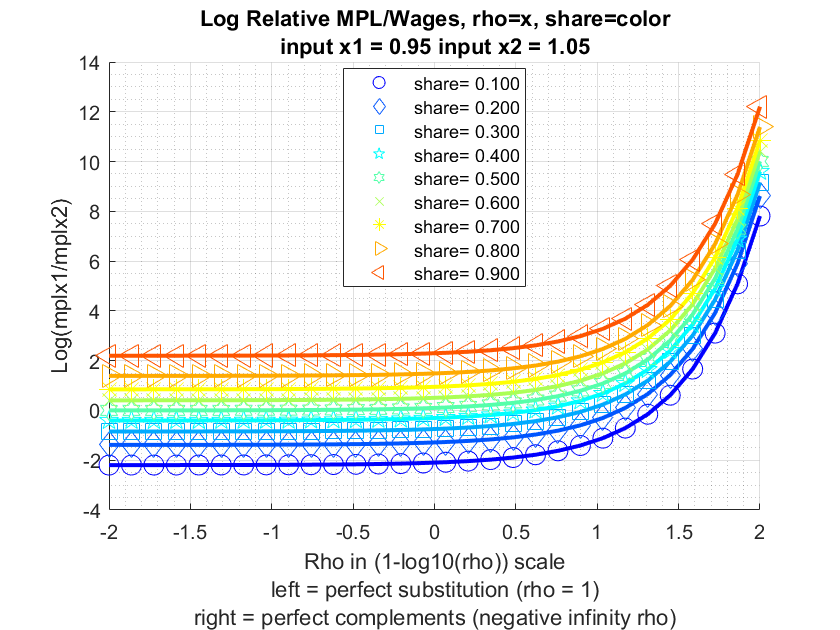
\includegraphics[width=5.20833in,height=\textheight]{img/bfwx_crs_nested_ces_mpl_images/figure_0.png}

\hypertarget{doubly-nest-layer-two-inputs-each-sub-nest-ces-problem}{%
\subsection{Doubly Nest Layer Two Inputs Each Sub-nest CES Problem}\label{doubly-nest-layer-two-inputs-each-sub-nest-ces-problem}}

In this third example, solve for optimal choices for a doubly nested
problem. Below, we first solve for the optimal choices, then we do a
number of checks, to make sure that the solutions are correct, as
expected.

\begin{verbatim}
% output requirement
fl_yz = 2.1;
% upper nest 0.1, lower nests 0.35 and -1 separately for rho values
cl_mn_prho = {[0.1], [0.35, -1]};
% unequal shares of share values
cl_mn_pshare = {[0.4], [0.3, 0.88]};
% differential wages
% in lower-left nest, not productive and very expensive, not very elastic
% last index for left or right. Values picked from demand problem parallel
% example.
cl_mn_yz_choices = {[nan, nan], [0.04789, 6.0934; 2.2044, 0.70496]};
% print option
bl_verbose = true;
[cl_mn_yz_choices, cl_mn_mpl_price] = ...
    bfw_crs_nested_ces_mpl(cl_mn_prho, cl_mn_pshare, cl_mn_yz_choices, ...
    mp_func, bl_verbose, bl_bfw_model);

----------------------------------------
xxxxxxxxxxxxxxxxxxxxxxxxxxxxxxxxxxxxxxxx
CONTAINER NAME: mp_container_map ND Array (Matrix etc)
xxxxxxxxxxxxxxxxxxxxxxxxxxxxxxxxxxxxxxxx
                    i    idx    ndim    numel    rowN    colN     sum       mean        std      coefvari      min        max  
                    _    ___    ____    _____    ____    ____    ______    _______    _______    ________    _______    _______

    mpl_price_c1    1     1      2        2       1       2      1.0206    0.51032    0.27499    0.53886     0.31587    0.70476
    mpl_price_c2    2     2      2        4       2       2      2.3618    0.59045     0.5082    0.86069     0.13121     1.3121
    prho_c2         3     4      2        2       1       2       -0.65     -0.325    0.95459    -2.9372          -1       0.35
    pshare_c2       4     6      2        2       1       2        1.18       0.59    0.41012    0.69512         0.3       0.88
    yz_c1           5     7      2        2       1       2      4.4862     2.2431    0.68863      0.307      1.7562       2.73
    yz_c2           6     8      2        4       2       2      9.0507     2.2627     2.7086     1.1971     0.04789     6.0934

xxx TABLE:mpl_price_c1 xxxxxxxxxxxxxxxxxx
            c1         c2   
          _______    _______

    r1    0.31587    0.70476

xxx TABLE:mpl_price_c2 xxxxxxxxxxxxxxxxxx
            c1         c2   
          _______    _______

    r1     1.3121    0.13121
    r2    0.39362    0.52484

xxx TABLE:prho_c2 xxxxxxxxxxxxxxxxxx
           c1     c2
          ____    __

    r1    0.35    -1

xxx TABLE:pshare_c2 xxxxxxxxxxxxxxxxxx
          c1      c2 
          ___    ____

    r1    0.3    0.88

xxx TABLE:yz_c1 xxxxxxxxxxxxxxxxxx
           c1       c2  
          ____    ______

    r1    2.73    1.7562

xxx TABLE:yz_c2 xxxxxxxxxxxxxxxxxx
            c1         c2   
          _______    _______

    r1    0.04789     6.0934
    r2     2.2044    0.70496

----------------------------------------
xxxxxxxxxxxxxxxxxxxxxxxxxxxxxxxxxxxxxxxx
CONTAINER NAME: mp_container_map Scalars
xxxxxxxxxxxxxxxxxxxxxxxxxxxxxxxxxxxxxxxx
                 i    idx    value
                 _    ___    _____

    prho_c1      1     3      0.1 
    pshare_c1    2     5      0.4 

% there are four optimal choices, they are
fl_mpl_x11 = cl_mn_mpl_price{2}(1,1);
fl_mpl_x12 = cl_mn_mpl_price{2}(1,2);
fl_mpl_x21 = cl_mn_mpl_price{2}(2,1);
fl_mpl_x22 = cl_mn_mpl_price{2}(2,2);
% display
st_print = strjoin(...
    ["completed double nest test:", ...
    ['nest 1 input 1, fl_mpl_x11=' num2str(fl_mpl_x11)], ...
    ['nest 1 input 2, fl_mpl_x12=' num2str(fl_mpl_x12)], ...
    ['nest 2 input 1, fl_mpl_x21=' num2str(fl_mpl_x21)], ...
    ['nest 2 input 2, fl_mpl_x22=' num2str(fl_mpl_x22)], ...
    ['nest 1 input 1, fl_mpl_x11/fl_mpl_x11=' num2str(fl_mpl_x11/fl_mpl_x11)], ...
    ['nest 1 input 2, fl_mpl_x12/fl_mpl_x11=' num2str(fl_mpl_x12/fl_mpl_x11)], ...
    ['nest 2 input 1, fl_mpl_x21/fl_mpl_x11=' num2str(fl_mpl_x21/fl_mpl_x11)], ...
    ['nest 2 input 2, fl_mpl_x22/fl_mpl_x11=' num2str(fl_mpl_x22/fl_mpl_x11)], ...    
    ], ";");
st_out = st_print;
ar_ch_out = char(strsplit(st_print,";")');
disp(ar_ch_out);

completed double nest test:                   
nest 1 input 1, fl_mpl_x11=1.3121             
nest 1 input 2, fl_mpl_x12=0.13121            
nest 2 input 1, fl_mpl_x21=0.39362            
nest 2 input 2, fl_mpl_x22=0.52484            
nest 1 input 1, fl_mpl_x11/fl_mpl_x11=1       
nest 1 input 2, fl_mpl_x12/fl_mpl_x11=0.099995
nest 2 input 1, fl_mpl_x21/fl_mpl_x11=0.29998 
nest 2 input 2, fl_mpl_x22/fl_mpl_x11=0.39999 
\end{verbatim}

\hypertarget{bfw-2022-nested-three-branch-four-layer-problem-mpl}{%
\subsection{BFW (2022) Nested Three Branch (Four Layer) Problem (MPL)}\label{bfw-2022-nested-three-branch-four-layer-problem-mpl}}

The model BFW 2022 has three branches and four layers. one of the
branches go down only three layers, the other two branches go down four
layers.

First, we prepare the various inputs:

\begin{verbatim}
% Controls
bl_verbose = true;
bl_bfw_model = true;

% Given rho and beta, solve for equilibrium quantities
mp_func = bfw_mp_func_demand();

% Following instructions in: PrjFLFPMexicoBFW\solvedemand\README.md

% Nests/layers
it_nests = 4;

% Input cell of mn matrixes
it_prho_cl = 1;
it_pshare_cl = 2;
it_yz_share_cl = 3;
for it_cl_ctr = [1,2,3]

    cl_mn_cur = cell(it_nests,1);

    % Fill each cell element with NaN mn array
    for it_cl_mn = 1:it_nests

        bl_yz_share = (it_cl_ctr == it_yz_share_cl);

        if (~bl_yz_share && it_cl_mn == 1)
            mn_nan = NaN;
        elseif (~bl_yz_share && it_cl_mn == 2) || (bl_yz_share && it_cl_mn == 1)
            mn_nan = [NaN, NaN];
        elseif (~bl_yz_share && it_cl_mn == 3) || (bl_yz_share && it_cl_mn == 2)
            mn_nan = NaN(2,2);
        elseif (~bl_yz_share && it_cl_mn == 4) || (bl_yz_share && it_cl_mn == 3)
            mn_nan = NaN(2,2,2);
        elseif (~bl_yz_share && it_cl_mn == 5) || (bl_yz_share && it_cl_mn == 4)
            mn_nan = NaN(2,2,2,2);
        elseif (~bl_yz_share && it_cl_mn == 6) || (bl_yz_share && it_cl_mn == 5)
            mn_nan = NaN(2,2,2,2,2);
        end
        cl_mn_cur{it_cl_mn} = mn_nan;
    end

    % Name cell arrays
    if (it_cl_ctr == it_prho_cl)
        cl_mn_prho = cl_mn_cur;
    elseif (it_cl_ctr == it_pshare_cl)
        cl_mn_pshare = cl_mn_cur;
    elseif (it_cl_ctr == it_yz_share_cl)
        cl_mn_yz_choices = cl_mn_cur;
    end
end

% Initialize share matrix
rng(123);
for it_cl_mn = 1:it_nests
    mn_pshare = cl_mn_pshare{it_cl_mn};
    if it_cl_mn == 4
        mn_pshare(2,:,:) = rand(2,2);
    else
        mn_pshare = rand(size(mn_pshare));
    end
    cl_mn_pshare{it_cl_mn} = mn_pshare;
end

% Initialize rho matrix
rng(456);
for it_cl_mn = 1:it_nests
    mn_prho = cl_mn_prho{it_cl_mn};
    if it_cl_mn == 4
        mn_prho(2,:,:) = rand(2,2);
    else
        mn_prho = rand(size(mn_prho));
    end
    % Scalling rho between 0.7500 and -3.0000
    % 1 - 2.^(linspace(-2,2,5))
    mn_prho = 1 - 2.^(mn_prho*(4) - 2);
    cl_mn_prho{it_cl_mn} = mn_prho;
end

% Initialize quantities matrix
rng(789);
for it_cl_mn = 1:it_nests
    mn_yz_choices = cl_mn_yz_choices{it_cl_mn};
    if it_cl_mn == 3
        mn_yz_choices(1,:,:) = rand(2,2);
    elseif it_cl_mn == 4
        mn_yz_choices(2,:,:,:) = rand(2,2,2);
    end
    % Scalling quantities between 3 amd 5
    mn_yz_choices = mn_yz_choices*(2) + 3;
    cl_mn_yz_choices{it_cl_mn} = mn_yz_choices;
end

% Initialize yz matrix
rng(101112);
\end{verbatim}

Second, display created inputs:

\begin{verbatim}
celldisp(cl_mn_prho);


cl_mn_prho{1} =
 
    0.5017



cl_mn_prho{2} =
 
    0.6071   -1.1955



cl_mn_prho{3} =
 
   -1.3523   -0.3346
   -0.4167   -1.9136



cl_mn_prho{4} =
 

(:,:,1) =

       NaN       NaN
   -1.0512    0.5869


(:,:,2) =

       NaN       NaN
    0.6209    0.1633



celldisp(cl_mn_pshare);


cl_mn_pshare{1} =
 
    0.6965



cl_mn_pshare{2} =
 
    0.2861    0.2269



cl_mn_pshare{3} =
 
    0.5513    0.4231
    0.7195    0.9808



cl_mn_pshare{4} =
 

(:,:,1) =

       NaN       NaN
    0.6848    0.4809


(:,:,2) =

       NaN       NaN
    0.3921    0.3432



celldisp(cl_mn_yz_choices);


cl_mn_yz_choices{1} =
 
   NaN   NaN



cl_mn_yz_choices{2} =
 
   NaN   NaN
   NaN   NaN



cl_mn_yz_choices{3} =
 

(:,:,1) =

    3.6467    3.4605
       NaN       NaN


(:,:,2) =

    4.5876    4.2488
       NaN       NaN



cl_mn_yz_choices{4} =
 

(:,:,1,1) =

       NaN       NaN
    4.9508    4.5178


(:,:,2,1) =

       NaN       NaN
    3.0212    3.0495


(:,:,1,2) =

       NaN       NaN
    3.2221    4.0763


(:,:,2,2) =

       NaN       NaN
    3.0909    4.1031
\end{verbatim}

Third, call function and solve for optimal demand:

\begin{verbatim}
% Call function
[cl_mn_yz_choices, cl_mn_mpl_price] = ...
    bfw_crs_nested_ces_mpl(cl_mn_prho, cl_mn_pshare, cl_mn_yz_choices, ...
    mp_func, bl_verbose, bl_bfw_model);

----------------------------------------
xxxxxxxxxxxxxxxxxxxxxxxxxxxxxxxxxxxxxxxx
CONTAINER NAME: mp_container_map ND Array (Matrix etc)
xxxxxxxxxxxxxxxxxxxxxxxxxxxxxxxxxxxxxxxx
                    i     idx    ndim    numel    rowN    colN      sum         mean        std       coefvari       min         max   
                    __    ___    ____    _____    ____    ____    ________    ________    ________    ________    _________    ________

    mpl_price_c1     1     1      2        2       1       2        1.0002      0.5001     0.28686     0.57362      0.29725     0.70294
    mpl_price_c2     2     2      2        4       2       2        1.0009     0.25022     0.17949     0.71731     0.080381     0.50351
    mpl_price_c3     3     3      3        8       2       4        1.0088      0.1261     0.10191     0.80822    0.0063057     0.25809
    mpl_price_c4     4     4      4       16       2       8           NaN         NaN         NaN         NaN    0.0025507     0.11203
    prho_c2          5     6      2        2       1       2      -0.58844    -0.29422      1.2746     -4.3323      -1.1955     0.60709
    prho_c3          6     7      2        4       2       2       -4.0173     -1.0043     0.76195    -0.75868      -1.9136    -0.33464
    prho_c4          7     8      3        8       2       4           NaN         NaN         NaN         NaN      -1.0512     0.62089
    pshare_c2        8    10      2        2       1       2       0.51299      0.2565    0.041923     0.16344      0.22685     0.28614
    pshare_c3        9    11      2        4       2       2        2.6747     0.66866     0.24087     0.36023      0.42311     0.98076
    pshare_c4       10    12      3        8       2       4           NaN         NaN         NaN         NaN      0.34318     0.68483
    yz_c1           11    13      2        2       1       2        8.0897      4.0448       0.173     0.04277       3.9225      4.1672
    yz_c2           12    14      2        4       2       2        16.015      4.0039     0.19166     0.04787       3.8468      4.2727
    yz_c3           13    15      3        8       2       4        31.235      3.9044     0.51337     0.13149       3.0635      4.5876
    yz_c4           14    16      4       16       2       8           NaN         NaN         NaN         NaN       3.0212      4.9508

xxx TABLE:mpl_price_c1 xxxxxxxxxxxxxxxxxx
            c1         c2   
          _______    _______

    r1    0.70294    0.29725

xxx TABLE:mpl_price_c2 xxxxxxxxxxxxxxxxxx
             c1         c2   
          ________    _______

    r1     0.19946    0.50351
    r2    0.080381    0.21754

xxx TABLE:mpl_price_c3 xxxxxxxxxxxxxxxxxx
             c1         c2          c3          c4    
          ________    _______    ________    _________

    r1     0.13727    0.24893    0.065108      0.25809
    r2    0.050551    0.21139    0.031132    0.0063057

xxx TABLE:mpl_price_c4 xxxxxxxxxxxxxxxxxx
            c1          c2          c3          c4           c5         c6          c7          c8    
          _______    ________    ________    _________    ________    _______    ________    _________

    r1        NaN         NaN         NaN          NaN         NaN        NaN         NaN          NaN
    r2    0.02507    0.099481    0.012272    0.0025507    0.027845    0.11203    0.018861    0.0038085

xxx TABLE:prho_c2 xxxxxxxxxxxxxxxxxx
            c1         c2   
          _______    _______

    r1    0.60709    -1.1955

xxx TABLE:prho_c3 xxxxxxxxxxxxxxxxxx
             c1          c2   
          ________    ________

    r1     -1.3523    -0.33464
    r2    -0.41668     -1.9136

xxx TABLE:prho_c4 xxxxxxxxxxxxxxxxxx
            c1         c2         c3         c4   
          _______    _______    _______    _______

    r1        NaN        NaN        NaN        NaN
    r2    -1.0512    0.58694    0.62089    0.16334

xxx TABLE:pshare_c2 xxxxxxxxxxxxxxxxxx
            c1         c2   
          _______    _______

    r1    0.28614    0.22685

xxx TABLE:pshare_c3 xxxxxxxxxxxxxxxxxx
            c1         c2   
          _______    _______

    r1    0.55131    0.42311
    r2    0.71947    0.98076

xxx TABLE:pshare_c4 xxxxxxxxxxxxxxxxxx
            c1         c2         c3         c4   
          _______    _______    _______    _______

    r1        NaN        NaN        NaN        NaN
    r2    0.68483    0.48093    0.39212    0.34318

xxx TABLE:yz_c1 xxxxxxxxxxxxxxxxxx
            c1        c2  
          ______    ______

    r1    3.9225    4.1672

xxx TABLE:yz_c2 xxxxxxxxxxxxxxxxxx
            c1        c2  
          ______    ______

    r1    4.0073    3.8887
    r2    3.8468    4.2727

xxx TABLE:yz_c3 xxxxxxxxxxxxxxxxxx
            c1        c2        c3        c4  
          ______    ______    ______    ______

    r1    3.6467    3.4605    4.5876    4.2488
    r2      4.23    4.2863    3.0635    3.7118

xxx TABLE:yz_c4 xxxxxxxxxxxxxxxxxx
            c1        c2        c3        c4        c5        c6        c7        c8  
          ______    ______    ______    ______    ______    ______    ______    ______

    r1       NaN       NaN       NaN       NaN       NaN       NaN       NaN       NaN
    r2    4.9508    4.5178    3.0212    3.0495    3.2221    4.0763    3.0909    4.1031

----------------------------------------
xxxxxxxxxxxxxxxxxxxxxxxxxxxxxxxxxxxxxxxx
CONTAINER NAME: mp_container_map Scalars
xxxxxxxxxxxxxxxxxxxxxxxxxxxxxxxxxxxxxxxx
                 i    idx     value 
                 _    ___    _______

    prho_c1      1     5     0.50172
    pshare_c1    2     9     0.69647
\end{verbatim}

\hypertarget{appendix-appendix}{%
\appendix}


\hypertarget{index-and-code-links}{%
\chapter{Index and Code Links}\label{index-and-code-links}}

\hypertarget{introduction-links}{%
\section{Introduction links}\label{introduction-links}}

\begin{enumerate}
\def\labelenumi{\arabic{enumi}.}
\tightlist
\item
  \href{https://fanwangecon.github.io/PrjLabEquiBFW/PrjLabEquiBFW/doc/intro/htmlpdfm/bfwx_intro.html}{The Labor Demand and Supply Problem}: \href{https://github.com/FanWangEcon/PrjLabEquiBFW/blob/main/PrjLabEquiBFW/doc/intro/bfwx_intro.mlx}{\textbf{mlx}} \textbar{} \href{https://github.com/FanWangEcon/PrjLabEquiBFW/blob/main/PrjLabEquiBFW/doc/intro/htmlpdfm/bfwx_intro.m}{\textbf{m}} \textbar{} \href{https://github.com/FanWangEcon/PrjLabEquiBFW/blob/main/PrjLabEquiBFW/doc/intro/htmlpdfm/bfwx_intro.pdf}{\textbf{pdf}} \textbar{} \href{https://fanwangecon.github.io/PrjLabEquiBFW/PrjLabEquiBFW/doc/intro/htmlpdfm/bfwx_intro.html}{\textbf{html}}

  \begin{itemize}
  \tightlist
  \item
    The Labor Demand and Supply Problem
  \end{itemize}
\end{enumerate}

\hypertarget{core-functions-links}{%
\section{Core Functions links}\label{core-functions-links}}

\begin{enumerate}
\def\labelenumi{\arabic{enumi}.}
\tightlist
\item
  \href{https://fanwangecon.github.io/PrjLabEquiBFW/PrjLabEquiBFW/doc/func/htmlpdfm/bfwx_mp_func_demand.html}{CES Demand Core Functions}: \href{https://github.com/FanWangEcon/PrjLabEquiBFW/blob/main/PrjLabEquiBFW/doc/func/bfwx_mp_func_demand.mlx}{\textbf{mlx}} \textbar{} \href{https://github.com/FanWangEcon/PrjLabEquiBFW/blob/main/PrjLabEquiBFW/doc/func/htmlpdfm/bfwx_mp_func_demand.m}{\textbf{m}} \textbar{} \href{https://github.com/FanWangEcon/PrjLabEquiBFW/blob/main/PrjLabEquiBFW/doc/func/htmlpdfm/bfwx_mp_func_demand.pdf}{\textbf{pdf}} \textbar{} \href{https://fanwangecon.github.io/PrjLabEquiBFW/PrjLabEquiBFW/doc/func/htmlpdfm/bfwx_mp_func_demand.html}{\textbf{html}}

  \begin{itemize}
  \tightlist
  \item
    This function generates a container map with key CES demand-side equation for a particular sub-nest.
  \item
    \textbf{PrjLabEquiBFW}: \emph{\href{https://github.com/FanWangEcon/PrjLabEquiBFW/blob/main/PrjLabEquiBFW/func/bfw_mp_func_demand.m}{bfw\_mp\_func\_demand()}}
  \end{itemize}
\end{enumerate}

\hypertarget{demand-links}{%
\section{Demand links}\label{demand-links}}

\begin{enumerate}
\def\labelenumi{\arabic{enumi}.}
\tightlist
\item
  \href{https://fanwangecon.github.io/PrjLabEquiBFW/PrjLabEquiBFW/doc/solvedemand/htmlpdfm/bfwx_crs_nested_ces.html}{Solve Nested CES Optimal Demand (CRS)}: \href{https://github.com/FanWangEcon/PrjLabEquiBFW/blob/main/PrjLabEquiBFW/doc/solvedemand/bfwx_crs_nested_ces.mlx}{\textbf{mlx}} \textbar{} \href{https://github.com/FanWangEcon/PrjLabEquiBFW/blob/main/PrjLabEquiBFW/doc/solvedemand/htmlpdfm/bfwx_crs_nested_ces.m}{\textbf{m}} \textbar{} \href{https://github.com/FanWangEcon/PrjLabEquiBFW/blob/main/PrjLabEquiBFW/doc/solvedemand/htmlpdfm/bfwx_crs_nested_ces.pdf}{\textbf{pdf}} \textbar{} \href{https://fanwangecon.github.io/PrjLabEquiBFW/PrjLabEquiBFW/doc/solvedemand/htmlpdfm/bfwx_crs_nested_ces.html}{\textbf{html}}

  \begin{itemize}
  \tightlist
  \item
    This function solves optimal choices given CES production function under cost minimization.
  \item
    Works with Constant Elasticity of Substitution problems with constant returns, up to four nest layers, and two inputs in each sub-nest.
  \item
    Takes as inputs share and elasticity parameters across layers of sub-nests, as well as input unit costs at the bottom-most layer.
  \item
    Works with Constant Elasticity of Substitution problems with constant returns, up to four nest layers, and two inputs in each sub-nest.
  \item
    \textbf{PrjLabEquiBFW}: \emph{\href{https://github.com/FanWangEcon/PrjLabEquiBFW/blob/main/PrjLabEquiBFW/solvedemand/bfw_crs_nested_ces.m}{bfw\_crs\_nested\_ces()}}
  \end{itemize}
\item
  \href{https://fanwangecon.github.io/PrjLabEquiBFW/PrjLabEquiBFW/doc/solvedemand/htmlpdfm/bfwx_crs_nested_ces_mpl.html}{Compute Nested CES MPL Given Demand (CRS)}: \href{https://github.com/FanWangEcon/PrjLabEquiBFW/blob/main/PrjLabEquiBFW/doc/solvedemand/bfwx_crs_nested_ces_mpl.mlx}{\textbf{mlx}} \textbar{} \href{https://github.com/FanWangEcon/PrjLabEquiBFW/blob/main/PrjLabEquiBFW/doc/solvedemand/htmlpdfm/bfwx_crs_nested_ces_mpl.m}{\textbf{m}} \textbar{} \href{https://github.com/FanWangEcon/PrjLabEquiBFW/blob/main/PrjLabEquiBFW/doc/solvedemand/htmlpdfm/bfwx_crs_nested_ces_mpl.pdf}{\textbf{pdf}} \textbar{} \href{https://fanwangecon.github.io/PrjLabEquiBFW/PrjLabEquiBFW/doc/solvedemand/htmlpdfm/bfwx_crs_nested_ces_mpl.html}{\textbf{html}}

  \begin{itemize}
  \tightlist
  \item
    Given labor quantity demanded, using first-order relative optimality conditions, find the marginal product of labor given CES production function.
  \item
    Takes as inputs share and elasticity parameters across layers of sub-nests, as well as quantity demanded at each bottom-most CES nest layer.
  \item
    Works with Constant Elasticity of Substitution problems with constant returns, up to four nest layers, and two inputs in each sub-nest.
  \item
    Allows for uneven branches, so that some branches go up to four layers, but others have less layers, works with BFW (2022) nested labor input problem.
  \item
    \textbf{PrjLabEquiBFW}: \emph{\href{https://github.com/FanWangEcon/PrjLabEquiBFW/blob/main/PrjLabEquiBFW/solvedemand/bfw_crs_nested_ces_mpl.m}{bfw\_crs\_nested\_ces\_mpl()}}
  \end{itemize}
\end{enumerate}

  \bibliography{book.bib,packages.bib}

\end{document}
